\subsection{Investigation of antennas}
\subsubsection{Conceptual framework and modeling}

\todo[inline]{Einige Themen hier sollten zum Theorieteil voriger Kapitel verschoben werden.}

\begin{figure}[h]
	\centering
	\includegraphics[width=0.7\linewidth]{content/img/antenna_port}
	\caption{Geometry of an antenna's feedpoint used in simulation. The antenna is fed through a waveport. This geometry leads to a port impedance of $50\,\Omega$.}
	\label{fig:antennaport}
\end{figure}


The coupling of various electrically small antennas placed in a TEM cell is investigated. Their electric and magnetic coupling is investigated through dipole moments. All antennas are fed with a power of 1\,W. Their material are made of a perfect electric conductor. Different positions and offsets are investigated and the results discussed. They are fed through a round wave port with a diameter of 0.46\,mm, and their wire has a diameter of 0.2\,mm and free-space permittivity. This results in a reference impedance of $Z_0\approx 50$\,$\Omega$. The TEM cell used has a width of $a=40$\,mm, a height of $b=24$\,mm and a length of $l=100$\,mm, and its cells walls and septum consist of a perfect electric conductor, too. The TEM cell model does not contain the tapered sections at the ports. The ports have an impedance of $50\,\Omega$ due to the TEM cell's geometry.


\begin{figure}[htbp]
	\centering
	\begin{subfigure}[b]{0.48\textwidth}
	\centering
\includegraphics[width=1\linewidth]{content/img/tem_cell_front}
\caption{xy-plane}
\label{fig:temcellfront}
	\end{subfigure}
	\hfill
	\begin{subfigure}[b]{0.48\textwidth}
	\centering
\includegraphics[width=1\linewidth]{content/img/tem_cell_side}
\caption{yz-plane}
\label{fig:temcellside}
	\end{subfigure}
	
	\caption{Geometrical arrangement of the TEM cell used in simulations. The front shows the xy-plane, and the side the yz-plane of the TEM cell.}
	\label{fig:example}
\end{figure}

The capacitance and inductance of the TEM cell is derived by calculating the feed current and voltage out of the S-parameters. The capacitance and inductance are then derived through the electric and magnetic peak energy. The values fluctuate slightly over frequency by $\pm1\,\%$, which is likely due to numerical inaccuracies. The average capacitance and inductance values over the frequency range are chosen. It is therefore assumed that the TEM cell has a constant capacitance and inductance. $C_T = 6.74\,\mathrm{pF}$, $L_T = 16.25\,\mathrm{nH}$. 

The coupling between the antenna and the two ports of the TEM cell are described by S-parameters, specifically the forward transmission coefficients $S_{\mathrm{A1}}$ and $S_{\mathrm{A2}}$. The magnitude of this coefficient is the same for the antenna to both ports ($|S_{\mathrm{A1}}|=|S_{\mathrm{A2}}|$). The power transferred from the antenna $P_{\mathrm{Antenna}}$ to the output ports $P_{\mathrm{Out1}}$ and $P_{\mathrm{Out2}}$ is then derived through

\begin{equation}
	P_{\mathrm{Antenna}}=\frac{P_{\mathrm{Out1}}}{10^{|S_{\mathrm{A1}}|/10}}=\frac{P_{\mathrm{Out2}}}{10^{|S_{\mathrm{A2}}|/10}}.
	\label{eqn:power_antenna}
\end{equation}

The fields are normalized such that 

\begin{equation}
	\iint_S \mathbf{E}^\pm \times \mathbf{H	_0}\pm \cdot d\mathbf{s}' = 1,
	\label{eqn:normalization of fields}
\end{equation}

where the surface $S$ spans over one of the output ports. The fields are linearly scaled by the complex coefficients $a$ and $b$. If only the TEM mode is considered, only one such pair of coefficients is needed to describe the fields at the output ports. Some investigations explicitly include the propagation of higher order modes. In this case, each mode is assigned a separate pair of coefficients $a_n$, $b_n$. The coefficients $a$ and $b$ have the unit $\sqrt{\mathrm{W}}$.

%\begin{figure}[h]
%	\centering
%	\includegraphics[width=1\linewidth]{content/img/sketch_dipoles_tem_cell.png}
%	\caption{Dipole moments and measurement point of $e_{0,z}$ in TEM cell}
%	\label{fig:sketch_dipoles_tem_cell2}
%\end{figure}

The coefficients $a$ and $b$ have the unit $\sqrt{\mathrm{W}}$. The fields $\mathbf{e_0}$ and $\mathbf{h_0}$ for a TEM cell is known \todo{Some plot or table for explanation}.The normalization condition leads to an output power equal to $P_\mathrm{out,1} = |a|^2/2$ and $P_\mathrm{out,2}=|b|^2/2$, which is also found in \cite{4091811}. This is derived by

\begin{subequations}
	\begin{equation}
		P_{\mathrm{out1}}=\iint_S \langle \mathbf{S} \rangle \cdot \mathrm{d}\mathbf{s'}= \iint_S \frac{1}{2} \, \Re \{ \left(a\cdot \mathbf{E}^\pm\right) \times \left(a\cdot \mathbf{H}^\pm\right)^* \}\cdot \mathrm{d}\mathbf{s'} = \frac{|a|^2}{2},
		\label{eqn:power_of_poynting1}
	\end{equation}
	\begin{equation}
		P_{\mathrm{out2}}=\iint_S \langle \mathbf{S} \rangle \cdot \mathrm{d}\mathbf{s'}= \iint_S \frac{1}{2} \, \Re \{ \left(b\cdot \mathbf{E}^\pm\right) \times \left(b\cdot \mathbf{H}^\pm\right)^* \}\cdot \mathrm{d}\mathbf{s'} = \frac{|b|^2}{2}.
		\label{eqn:power_of_poynting2}
	\end{equation}
\end{subequations}

Because ideal TEM fields are assumed at the output ports, the Poynting vector has no imaginary component,


\begin{equation}
	\mathbf{E}^\pm\times\mathbf{H}^\pm=\Re\{\mathbf{E^\pm}\times\left(\mathbf{H}^\pm\right)^*\} \quad\text{for TEM mode}.
	\label{eqn:equivalent_tem}
\end{equation}

Consequently, if the normalized electric field distribution of the TEM mode $\mathbf{E^\pm}$ is unknown, it may be derived by setting the output power of a waveport to $P_{\mathrm{out}}=1/2\,\mathrm{W}$, where $|a|=|b|=1\,\sqrt{\mathrm{W}}$. For example, the uniformly distributed, normalized electric field along the y-axis in the center of the TEM cell ($z=0$, $x=0$) is derived by

\begin{equation}
	|a|\cdot\mathbf{E}^\pm(0,y,0)=1\sqrt{\mathrm{W}}\cdot\mathbf{E}^\pm = \frac{\sqrt{P_\mathrm{out}R_\mathrm{waveport}}}{b/2}
\end{equation}
 
 The difference in phase of $S_{\mathrm{A1}}$ and $S_{\mathrm{A2}}$ influence the quantity of magnetic dipole moments and electric dipole moments.  If the dipole moments are placed in the center of the TEM cell half-way between both output ports, they will contain the same power, therefore $|a| = |b|$. In this case, a phase shift of $\pi$ indicates the presence of a magnetic dipole moment and the absence of electric dipole moments. This is shown by

\begin{subequations}
	\begin{equation}
		\mathbf{m}_\mathrm{e} = \frac{a+b}{\mathbf{E}^\pm} = \frac{a+a\cdot e^{j\pi}}{\mathbf{E}^\pm} = 0,
	\end{equation}
	\begin{equation}
		\mathbf{m}_\mathrm{m} = j\frac{a-b}{\mathbf{E}^\pm\cdot k_0} = j\frac{a-a\cdot e^{j\pi}}{\mathbf{E}^\pm\cdot k_0} = j\frac{2a}{\mathbf{E}^\pm\cdot k_0}.
	\end{equation}
\end{subequations}

 A phase shift of zero indicates the opposite case. The influence of the electric and magnetic dipole moment is equal, if the phase shift equals $\pi/2$. 

If only the TEM mode propagates, only the y-component of an electric dipole moment and the x-component of a magnetic dipole moment generates output power, assuming they are centrally located ($x=0$, $y=b/4$, $z=0$). This is due to the magnetic field containing only an x-component $\mathbf{H}^\pm = H_x^\pm e^{\pm k_0 z}$, and the electric field only an y-component $\mathbf{E}^\pm = E_y^\pm e^{\pm k_0 z}$ at the center of the TEM cell. \todo{Sketch this situation. Also, $e^{\pm k_0 z}$ indicated that at z=0 the dipole moment is located. Consider this in all sketches}
An offset of dipole moments or propagation of higher order modes lead to different field components of $\mathbf{H}^\pm$ and $\mathbf{E}^\pm$, and therefore to a change in coupling. These effects are investigated numerically in \autoref{sec:dipole_moments}.

A magnetic dipole moment can be expressed equivalently as either an electric current loop or a magnetic line current, as described in \autoref{eqn:magn_current_curr_loop}. For infinitesimal magnetic dipoles, this duality simplifies to
\begin{equation}
	m_{\mathrm{m}}=j\omega\mu_0 m_{\mathrm{0}},
	\label{eqn:m_mymag_ifa}
\end{equation}
where $m_{\mathrm{m}}$ (in V$\cdot$m) denotes the magnetic dipole moment in the magnetic current representation, and $m_{\mathrm{0}}$ (in A$\cdot$m$^2$) denotes the moment in the electric current representation.

If the output power and phase shifts of the waveports are known, any antenna in the TEM cell may be replaced by an electric and a magnetic dipole moment. Using numeric simulation, the phase shift is determined by measuring the phase shifts of the electric fields at both output ports. When applying this described method in a measurement with a real TEM cell, the phase shift is found by adding and subtracting the output powers of both ports, as is shown in \cite{Sreenivasiah_Chang_Ma_1981}.

The energy density is given by \cite[p. 330]{Griffiths_2024}

\begin{equation}
	w_\mathrm{EM} = \frac{1}{2}\left(\underbrace{\epsilon E^2}_{\text{Electric energy} w_E} + \underbrace{\frac{1}{\mu} B ^ 2}_{\text{Magnetic energy} w_M}\right).
	\label{eqn:em_energy}
\end{equation}

Integrating $w_\mathrm{EM}$ over a volume yields the total electromagnetic energy in this volume. Similarly, integrating $w_E$ gives the electric energy in said volume, and $w_M$ the magnetic energy.

If all of the energy is provided by an electrically short antenna, its equivalent reactances can be derived through \cite[pp 107, 328]{Griffiths_2024}

\begin{subequations}
	\begin{equation}
		L = 2\frac{W_m}{I^2}
		\label{eqn:m_energy}
	\end{equation}
	\begin{equation}
		C = 2 \frac{W_e}{V^2}
		\label{eqn:e_energy}
	\end{equation}
\end{subequations}


All simulations are counterchecked by inserting frequency-dependent dipole moments and checking the power and phase of the output ports.

In the measurement configuration, the TEM cell with an inserted antenna can be modeled as a three-port network. The two output ports of the TEM cell are denoted as ports 1 and 2, while the antenna feed point is represented as port A. The behavior of this system is fully characterized by its scattering matrix, given as

\begin{equation}
	\left[S\right]=
	\begin{bmatrix}
		S_{11} & S_{12} & S_{1A} \\
		S_{21} & S_{22} & S_{2A} \\
		S_{A1} & S_{A2} & S_{A}
	\end{bmatrix}.
\end{equation}

 The current through the feedpoint of the antennas are calculated with those S-parameters,
 
 \begin{equation}
 	I_{in} = \sqrt{P_{in}}\frac{(1-S_{AA})}{\sqrt{Z_0}},
 \end{equation}
 
  $P_{in}$ is the power applied to the port, not considering reflections. The voltage at the feedpoint is calculated in a similar fashion as 
 
 \begin{equation}
 	V_{in} = \sqrt{P_{in}}(1-S_{AA})\sqrt{Z_0}.
 \end{equation}
 
 The impedance seen from the feedpoint is 
 
 \begin{equation}
 	Z_{in}=Z_0\frac{1+S_{AA}}{1-S_{AA}}.
 \end{equation}
 

\FloatBarrier
\subsubsection{Monopole Antenna}
\subsubsection{Setup}
\FloatBarrier

\begin{figure}[htbp]
	\centering
	\hspace*{-0.0cm}
	\begin{subfigure}[b]{0.48\textwidth}
		\centering
		\includegraphics[height=8cm]{content/img/monopole_near_field}
		\caption{}
		\label{fig:monopolenearfield}		
	\end{subfigure}
	\hfill
	\begin{subfigure}[b]{0.48\textwidth}
		
		\centering
		\raisebox{0.12cm}{\includegraphics[height=8cm]{content/img/monopole_antenna}}
		\caption{}
		\label{fig:monopoleantenna}
	\end{subfigure}
	
	\caption{Geometry of monopole antenna inserted into TEM cell with its electric near-field.}
	\label{fig:field_monopole_antenna}
\end{figure}


The monopole antenna, shown in \autoref{fig:monopoleantenna}, is installed at the center of the TEM cell and connected to the feedpoint located on the top wall. It has a length of 5\,mm, which makes it electrically short at frequencies up to 6\,GHz. It may be approximated as an infinitesimal electric dipole for frequencies up to 1.25\,GHz. The equivalent dipole moments $\mathbf{m}_e$ and $\mathbf{m}_m$ are derived through \cref{eqn:ifa_me, eqn:ifa_mm}. 

The frequency range investigated reaches from 1\,MHz to 3\,GHz. \autoref{fig:te01_te10_tem_propagation} demonstrates the cut-off frequencies of higher-order modes of the TEM cell in use for the simulation, where the cut-off frequency of TE\textsubscript{01} equals $f_{\mathrm{c,01}}=3.12\,\mathrm{GHz}$. The output power is influenced by the propagation of this evanescent mode, which must be considered in the simulation results in the upper frequency range. 


\FloatBarrier
\subsubsection{Equivalent dipole moments}
\FloatBarrier



The electric dipole moment is normalized to the free-space wave impedance to enable comparison with the magnetic dipole moment \cite{Kreindl_Bauernfeind_Weiss_Stockreiter_Kaltenbacher_2024}. The electric dipole moment shown in \autoref{fig:dipole_moments_monopole} increases approximately linearly over frequency, while the magnetic dipole moment is negligible over the whole frequency range. Consequently, the phase difference between the powers $\Delta = \varphi_2 - \varphi_1=0$ over the whole frequency range. 

\begin{figure}[htbp]
	\centering
	\begin{subfigure}[b]{0.48\textwidth}
		\centering
		\includegraphics[width=1\linewidth]{content/img/dipole_moments_monopole.png}
		\caption{Dipole moments}
		\label{fig:dipole_moments_monopole}
	\end{subfigure}
	\hfill
	\begin{subfigure}[b]{0.48\textwidth}
		\centering
		\includegraphics[width=1\linewidth]{content/img/phase_shift_monopole}
		\caption{Phase shift}
		\label{fig:phaseshiftmonopole}
	\end{subfigure}
	
	\caption{The equivalent dipole moments of the monopole antenna and the corresponding induced phase shift between the wave ports are presented in separate figures.}
	\label{fig:monopole_moments_phase}
\end{figure}

\FloatBarrier
\subsubsection{Electrical characteristics}
\FloatBarrier

\begin{figure}[htbp]
	\centering
	\begin{subfigure}[b]{0.48\textwidth}
		\centering
		\centering
		\includegraphics[width=1\linewidth]{content/img/monopole_feed_voltage}
		\caption{Voltage at feedpoint}
		\label{fig:monopolefeedvoltage}
	\end{subfigure}
	\hfill
	\begin{subfigure}[b]{0.48\textwidth}
		\centering
		\includegraphics[width=1\linewidth]{content/img/monopole_feed_current}
		\caption{Current at feedpoint}
		\label{fig:monopolefeedcurrent}
	\end{subfigure}
	
	\caption{Current and voltage at feedpoint of monopole antenna over frequency.}
	\label{fig:example}
\end{figure}

\todo{axis typo}

The electric current present in the monopole antenna is aligned with the electric field $\mathbf{e}_\mathrm{TEM}^\pm$ of the dominant TEM mode present in the investigated frequency range. Only the the electric dipole moment in y-direction and the magnetic dipole moment in x-direction are needed to model the antenna, because they align with the fields of the TEM mode.

According to \autoref{eqn:J1_propagating_waves}, this will lead to a coupling with the output ports. \autoref{eqn:J1_propagating_waves} also requires $\mathbf{e}_\mathrm{TEM}^\pm$ and the part of $I$ contributing to the output power to be in phase at the position of the monopole antenna, due to $\mathbf{e}_\mathrm{TEM}^\pm$ and $\mathbf{h}_\mathrm{TEM}^\pm$ being in-phase at the output ports. Using \cref{eqn:e_int_a, eqn:e_int_b} and integrating the current $I$ in \autoref{fig:monopolefeedcurrent} yields

\begin{equation}
	\mathbf{m}_e=\int_C \boldsymbol{\tau} I(l)\,dl = 82.00\,\mu\mathrm{Am}\cdot\mathbf{\hat{a}}_z,
\end{equation}

which is equivalent to $\mathbf{m_e}=3.09\cdot 10^{-2} \cdot\mathbf{\hat{a}}_z\,\mathrm{Vm}$, if normalized to the free-space wave impedance $Z_0\approx 376.73\,\Omega$. Since the monopole antenna is located in the center, $\mathbf{e}_\mathrm{TEM}^\pm$ remains constant over $y$.

%For example, measuring the y-component of the electric field at the center of output port 1 yields $E_y^+(x=0, y, z=l/2)=15.35\,\mathrm{V/m}$, which is constant over $y$. \todo{differentiate somehow between normalized and normal electric field}. Using the Lorentz Reciprocity theorem \autoref{eqn:J1_propagating_waves}, and integrating $E_y^+(x=0, y, z=l/2)$ and $I(x=0, y, z=l/2)$ over the length of the monopole antenna yields \todo{all values must be peak values}

%\begin{equation}
%	\int_C E_y^+(x=0, y, z=l/2)\cdot I(x=0, y, z=l/2)\,dy=521.9\,\mathrm{\mu W}=2a^2.
%\end{equation}
%
%Applying \autoref{eqn:ifa_me} to then derive the electric dipole moment leads to 
%
%\begin{equation}
%	\mathbf{m}_e = \sqrt{2}\frac{521.9\,\mathrm{W}}{\mathbf{E^\pm}}=
%\end{equation}




The voltage $V$ at the feedpoint in \autoref{fig:monopolefeedvoltage} remains largely constant over the frequency range. This agrees with the absence of magnetic dipole moment $\mathbf{m}_m$, which is directly related to induced voltage according to \autoref{eqn:m_v}. The current $I$ at the feedpoint in \autoref{fig:monopolefeedcurrent} rises linearly. According to \autoref{eqn:me_i}, the frequency behavior of $\mathbf{m}_\mathrm{e}$ is proportional to $I$. \autoref{eqn:me_i} cannot directly be applied using $I$, because some of this current returns as displacement current to the feedpoint (see \autoref{fig:monopolenearfield}), not contributing to the electric coupling. Furthermore, this agrees with the quadratically increasing output power in \autoref{fig:monopoleoutputpower} and the quadratically increasing radiation resistance determined.

\begin{figure}[htbp]
	\centering
	\begin{subfigure}[t]{0.48\textwidth}
		\centering
		\includegraphics[height=5cm]{content/img/monopole_output_power}
		\caption{Output electric field and power of monopole antenna.}
		\label{fig:monopoleoutputpower}
	\end{subfigure}
	\hfill
	\begin{subfigure}[t]{0.48\textwidth}
		\centering
		\includegraphics[height=5cm]{content/img/monopole_moment_comp}
		\caption{Comparison of output power produced by monopole antenna and equivalent dipole moments.}
		\label{fig:monopolemomentcomp}
	\end{subfigure}
	
	\caption{Output power and electric field data of antenna and equivalent dipole moments}
	\label{fig:monopole_power_comp}
\end{figure}

The derived equivalent dipole moments $\mathbf{m}_e$, $\mathbf{m}_m$ positioned in the center of the TEM cell produce output power shown in \autoref{fig:monopolemomentcomp}, where they are compared with the monopole antenna. The approximation with the dipole moments worsens, when approaching the cut-off frequency of the first higher-order mode. The coefficients $a_{01}$ and $b_{01}$ of the TE\textsubscript{01} have to be considered, which would provide the difference in power to increase accuracy.

The output power rises quadratically over the frequency, which fits the linearly rising electric dipole moment and the quadratically rising radiation resistance determined in section \todo{Fill in}.




\begin{figure}[htbp]
	\centering
	\begin{minipage}[t]{0.48\textwidth}
		\centering
		\centering
		\includegraphics[width=1\linewidth]{content/img/monopole_current_dist}
		\caption{At $3\,\mathrm{GHz}$}
		\label{fig:currentdistributionmonopole}
		\hfill
	\end{minipage}
	\hfill
	\begin{minipage}[t]{0.48\textwidth}
		\centering
		\includegraphics[width=1\linewidth]{content/img/current_loop_charge_distribution_1MHz}
		\caption{At $1\,\mathrm{MHz}$}
		\label{fig:currentloopchargedistribution1mhz}
	\end{minipage}
	\caption{Current distribution along the monopole antenna at frequencies $1\,\mathrm{MHz}$ and $3\,\mathrm{GHz}$}
	\label{fig:monopole_current_dist}
\end{figure}






The distribution of the current along the monopole antenna shown in \autoref{fig:monopole_current_dist} is numerically derived by integrating the magnetic field intensity in a closed loop around the antenna at each position. 

Near the feedpoint at $0\,\mathrm{mm}$ non-linearities become apparent, due to significant displacement current in this region, as \autoref{fig:monopolenearfield} makes clear. This causes the current in the antenna to rapidly decreases in this section. 

The current distribution at $3\,\mathrm{GHz}$ (see \autoref{fig:currentdistributionmonopole}) approximates that of a small electric dipole as described in \autoref{sec:small_electric_dipole}. It shows an approximately linear decrease. Any current observed beyond the antenna length of $5\,\mathrm{mm}$ is attributed to displacement current to the septum, as is visible by the increased electric field there in \autoref{fig:monopolenearfield}.

The current distribution at $1\,\mathrm{MHz}$ demonstrated in \autoref{fig:currentloopchargedistribution1mhz} approximately follows the behavior of an infinitesimal electric dipole discussed in \autoref{sec:infinitesimal_electric_dipoles}. There, the current remains nearly constant over some sections of antenna length, decreasing towards the end. Additionally, the magnitude of the current is significantly lower at this frequency. 

\begin{figure}
	\centering
	\includegraphics[width=0.4\linewidth]{content/img/monopole_imp}
	\caption{Magnitude and phase of monopole antenna's impedance.}
	\label{fig:monopoleimp}
\end{figure}


This frequency-dependent behavior is explained by the impedance of the monopole antenna shown in \autoref{fig:monopoleimp}. At low frequencies, the antenna impedance demonstrates a high magnitude, which rapidly decreases as frequency increases. Over the whole frequency range, it exhibits highly capacitive behavior, which is consistent with \autoref{eqn:compl_power_inf_elec_dipole}.


An equivalent circuit is derived in \autoref{fig:chucircuit}, which is known as Chu equivalent circuit for a short dipole \cite{Hansen_Collin_2013}. \todo{What is the purpose of this circuit here? Explain more. And should other chapters have circuits, too?}


\begin{figure}[htbp]
	\centering
	\includegraphics[width=0.3\linewidth]{content/img/chu_circuit}
	\caption{Chu equivalent circuit of short dipole}
	\label{fig:chucircuit}
\end{figure}

\FloatBarrier
\subsubsection{Current distribution on septum}
\FloatBarrier

\begin{figure}[h]
	\centering
	\includegraphics[width=1\linewidth]{content/img/monopole_surface_currents.png}
	\caption{Current surface density at 3\,GHz}
	\label{fig:monopole_surface_currents}
\end{figure}


\autoref{fig:monopole_surface_currents} shows the surface current density on the septum caused by the monopole antenna. The current heads towards output ports in-phase, which causes the output power to be in-phase, too. This is a characteristic of the dominant electric dipole moment, predicted by . 

\begin{figure}[h]
	\centering
	\includegraphics[width=1\linewidth]{content/img/monopole_surface_currents_te01.png}
	\caption{Current surface density at 3.3\,GHz }
	\label{fig:monopole_surface_current_te01}
\end{figure}

\autoref{fig:monopole_surface_current_te01} shows the current density of the septum at 3.3\,GHz. Due to the magnetic fields propagating in the z-direction, the current on the septum creates a pattern of swirls. Current, which reach an output ports by following this pattern, contributes to the total power transferred by the TE\textsubscript{01} mode.

\todo[inline]{idea: offset in z-direction, show surface current how it gets a pahse shift at waveports, and a magnetic dipole moment appears to be induced}.

\FloatBarrier
\subsubsection{Electromagnetic energy in the TEM cell}
\FloatBarrier

The antenna produces electromagnetic energy in the TEM cell, which is derived by \autoref{eqn:em_energy}. This gives information about the real and imaginary power consumed by the antenna. Furthermore, it is possible to derive the inductance and capacitance of the monopole antenna in the TEM cell through \cref{eqn:m_energy, eqn:e_energy}. With help of the peak electrical energy shown in \autoref{fig:monopole_em_energy}, the reactances turn out to be

\begin{subequations}
	\begin{equation}
		L = todo
	\end{equation}
	\begin{equation}
		C = todo
	\end{equation}
\end{subequations}
\todo{Problem: eqc has series circuit, for which must be accounted}

\begin{figure}[htbp]
	\centering
	\begin{subfigure}[b]{0.48\textwidth}
	\centering
\includegraphics[width=1\linewidth]{content/img/monopole_magn_energy}
\caption{Magnetic energy}
\label{fig:monopolemagenergy}
	\end{subfigure}
	\hfill
	\begin{subfigure}[b]{0.48\textwidth}
	\centering
\includegraphics[width=1\linewidth]{content/img/monopole_elec_energy}
\caption{Electric energy}
\label{fig:monopoleelecenergy}
	\end{subfigure}
	
	\caption{Peak electromagnetic energy in the TEM cell generated by the monopole antenna}
	\label{fig:monopole_em_energy}
\end{figure}

As discussed previously, the monopole antenna demonstrates capacitive behavior and has a lot of voltage. This leads to the electromagnetic energy to be predominantly electric.

\FloatBarrier

\subsection{Loop antenna}\label{sec:loop_sim}
\subsubsection{Setup}
\FloatBarrier

\begin{figure}[htbp]
	\centering
	\begin{subfigure}[b]{0.48\textwidth}
		\centering
		\includegraphics[width=1\linewidth]{content/img/loop_near_field}
		\caption{}
		\label{fig:loopnearfield}
	\end{subfigure}
	\hfill
	\begin{subfigure}[b]{0.48\textwidth}
		\centering
		\includegraphics[width=1\linewidth]{content/img/loop_antenna}
		\caption{}
		\label{fig:loopantenna}
	\end{subfigure}
	
	\caption{Geometry of loop antenna inserted into the TEM cell with its magnetic near-field. The return path leads into the conducting surface of the cell.}
	\label{fig:loop_moments_phase}
\end{figure}

A square loop antenna is placed in the TEM cell, each side has a length of 1.6\,mm. This is preferable to a round antenna in these numerical simulations, due to more accurate mesh modeling and clearer investigation of the resulting dipole moments. The normal vector of its surface points in x-direction.

\FloatBarrier
\subsubsection{Equivalent dipole moments}
\FloatBarrier

\begin{figure}[htbp]
	\centering
	\begin{subfigure}[b]{0.48\textwidth}
		\centering
		\includegraphics[width=1\linewidth]{content/img/dipole_moments_loop_antenna.png}
		\caption{Dipole moments}
		\label{fig:dipole_moments_loop_antenna}
	\end{subfigure}
	\hfill
	\begin{subfigure}[b]{0.48\textwidth}
		\centering
		\includegraphics[width=1\linewidth]{content/img/loop_phase}
		\caption{Phase}
		\label{fig:loopphase}
	\end{subfigure}
	
	\caption{Dipole moments and phase shift of loop antenna}
	\label{fig:loop_moments_phase}
\end{figure}

\FloatBarrier
\subsubsection{Electrical characteristics}
\FloatBarrier

\begin{figure}[htbp]
	\centering
	\begin{subfigure}[b]{0.45\textwidth}
	\centering
\includegraphics[width=1\linewidth]{content/img/loop_elec_energy}
\caption{Electric energy}
\label{fig:loopelecenergy}
	\end{subfigure}
	\hfill
	\begin{subfigure}[b]{0.45\textwidth}
	\centering
\includegraphics[width=1\linewidth]{content/img/loop_mag_energy}
\caption{Magnetic energy}
\label{fig:loopmagenergy}
	\end{subfigure}
	
	\caption{}
	\label{fig:example}
\end{figure}
 
%
%The output power is calculated through the S-parameters. The impedance too. The voltage and current at the antenna port follow from the impedance and input power. The magnetic and electric energy in the TEM cell is calculated through integrating the electric and magnetic field intensities. By dividing them with the voltage and current, the inductance and capacitance of the antenna is calculated.  \todo{Passt so vermutlich nicht: die port s parameter lügen diesbezüglich ein wenig, da sehr viel strom bereits nähe des ports als displacement current zurückfließt.}



\begin{figure}[htbp]
	\centering
	\begin{subfigure}[b]{0.45\textwidth}
	\centering
\includegraphics[width=1\linewidth]{content/img/loop_feed_current}
\caption{Current}
\label{fig:loopfeedcurrent}
	\end{subfigure}
	\hfill
	\begin{subfigure}[b]{0.45\textwidth}
	\centering
\includegraphics[width=1\linewidth]{content/img/loop_feed_voltage}
\caption{Voltage}
\label{fig:loopfeedvoltage}
	\end{subfigure}
	
	\caption{Voltage and current at feedpoint of the loop antenna.}
	\label{fig:example}
\end{figure}


If the current $I$ in the loop antenna was constant, the electric field integral in \autoref{eqn:ind_volt} would equal zero. However, this current varies along the loop as shown in \autoref{fig:loopfeedcurrent}, and much of it escapes as displacement current and leads to electric coupling. 

\autoref{fig:loopfeedvoltage} demonstrates the voltage at the feedpoint of the antenna, and it does resemble therefore the magnetic dipole moment in \autoref{fig:dipole_moments_loop_antenna} strongly. 


Using a similar line of argument, the electric dipole moment is derived by $j\omega C U$

\autoref{fig:eqc_balanis} shows an equivalent circuit for the electrically small loop antenna, where $C$ models stray capacitances, $R_L$ the losses, $R_r$ the radiation, $L_i$ the internal inductance and $L_A$ the external inductance \cite[p. 244] {Balanis_1997}. The model used in the simulation consists of a perfect conductor, therefore $R_L$ and $L_A$ are neglected. Instead, the simplified schematic in \autoref{fig:eqc_simple} is used, where $R_A$, $L_A$ and $C_A$ model the impedance behavior of the antenna.

\begin{figure}[htbp]
	\centering
	\begin{subfigure}[b]{0.45\textwidth}
	\centering
	\resizebox{0.7\textwidth}{!}{
	\begin{tikzpicture}
		% Paths, nodes and wires:
		\draw (11.75, 6) to[european inductor, l={$L_{i}$}] (9.75, 6);
		\draw (12, 2) to[european inductor, l_={$L_{A}$}] (12, 4);
		\draw (7, 6) to[capacitor, l={$C$}] (7, 2);
		\draw (12, 5.75) to[european resistor, l={$R_{r}$}] (12, 3.75);
		\draw (9.25, 6) to[european resistor, l={$R_{L}$}] (7.25, 6);
		\node[ground] at (7, 2){};
		\node[ground] at (12, 2){};
		\draw (7, 6) -- (5, 6);
		\node[circ] at (7, 6){};
		\draw (7, 6) -- (7.25, 6);
		\draw (9.25, 6) -- (10, 6);
		\draw (11.75, 6) -- (12, 6);
		\draw (12, 5.75) -| (12, 6);
		\draw[-latex] (5, 6.5) -- (6.75, 6.5);
		\node[shape=rectangle, minimum width=2.215cm, minimum height=0.965cm] at (6.534, 6.75){} node[anchor=north west, align=left, text width=1.827cm, inner sep=6pt] at (5.409, 7.25){$P_{in}$};
	\end{tikzpicture}
}
\caption{Full equivalent circuit}
\label{fig:eqc_balanis}

	\end{subfigure}
	\hfill
	\hspace*{-0.5cm}
	\begin{subfigure}[b]{0.45\textwidth}
	\centering
	\resizebox{0.65\textwidth}{!}{
	\begin{tikzpicture}
		% Paths, nodes and wires:
		\draw (11, 3) to[european inductor, l_={$L_{A}$}] (11, 5);
		\draw (7, 6) to[capacitor, l={$C_A$}] (7, 2);
		\node[ground] at (7, 2){};
		\node[ground] at (11, 2){};
		\draw (7, 6) -- (5, 6);
		\node[circ] at (7, 6){};
		\draw (7, 6) -- (7.25, 6);
		\draw[-latex] (5, 6.5) -- (6.75, 6.5);
		\node[shape=rectangle, minimum width=2.215cm, minimum height=0.965cm] at (6.534, 6.75){} node[anchor=north west, align=left, text width=1.827cm, inner sep=6pt] at (5.409, 7.25){$P_{in}$};
		\draw (11, 2) -| (11, 3);
		\draw (7.25, 6) to[european resistor, l={$R_A$}] (11, 6);
		\draw (11, 6) -- (11, 5);
	\end{tikzpicture}
}
\caption{Reduced equivalent circuit}
\label{fig:eqc_simple}
	\end{subfigure}
	
	\caption{A full equivalent circuit of the small loop antenna, and a simplified version of it}
	\label{fig:eqc_loop}
\end{figure}


\begin{figure}[htbp]
	\centering
	\resizebox{\textwidth}{!}{%
\begin{tikzpicture}
	% Paths, nodes and wires:
	\node[shape=circle, draw, line width=1pt, minimum width=0.965cm](N1) at (2.5, 9.5){} node[anchor=east] at (N1.west){$VI$};
	\node[ground] at (2.5, 8){};
	\draw (2.5, 9) -| (2.5, 8);
	\draw (4, 11) to[european resistor, l={$R_s$}] (6, 11);
	\draw (7.5, 11) to[capacitor, l={$C_A$}] (7.5, 8);
	\draw (10, 11) to[european inductor, l={$L_A$}] (10, 8);
	\node[ground] at (7.5, 8){};
	\node[ground] at (10, 8){};
	\draw (2.5, 10) -| (2.5, 11) -- (4, 11);
	\draw (6, 11) -- (7.5, 11) -- (10, 11);
	\node[circ] at (7.5, 11){};
	\node[circ] at (10.5, 10){};
	\node[shape=rectangle, draw, line width=1pt, dash pattern={on 4pt off 4pt}, minimum width=4.965cm, minimum height=4.465cm] at (8.5, 9.25){};
	\node[shape=rectangle, minimum width=5.215cm, minimum height=1.465cm] at (8.375, 11.5){} node[anchor=north west, align=left, text width=4.827cm, inner sep=6pt] at (5.75, 12.25){Antenna};
	\draw (10, 11) to[capacitor, l={$C_k$}] (14.5, 11);
	\node[circ] at (10, 11){};
	\draw (14.5, 10) to[european inductor, l={$L_{T2}$}] (18, 10);
	\draw (14.5, 12) to[european inductor, l={$L_{T1}$}] (18, 12);
	\draw (14.5, 10) -| (14.5, 12);
	\node[circ] at (14.5, 11){};
	\draw (18, 10) to[capacitor, l={$C_{T2}$}] (18, 8);
	\draw (23, 10) to[european resistor, l={$R_2$}] (23, 8);
	\node[ground] at (18, 8){};
	\node[ground] at (20.5, 8){};
	\node[circ] at (18, 10){};
	\draw (18, 12) -- (22, 12);
	\draw (20.5, 10) to[capacitor, l={$C_{T1}$}] (20.5, 8);
	\node[ground] at (23, 8){};
	\draw (25.5, 10) to[european resistor, l={$R_1$}] (25.5, 8);
	\node[ground] at (25.5, 8){};
	\draw (22, 12) -- (24.5, 12);
	\draw (20.5, 10) -- (20.5, 12);
	\node[jump crossing] at (20.5, 10){};
	\draw (18, 10) -- (20.36, 10);
	\draw (20.64, 10) -- (23, 10);
	\draw (24.5, 12) -| (25.5, 10);
	\node[circ] at (20.5, 12){};
	\node[shape=rectangle, draw, line width=1pt, dash pattern={on 4pt off 4pt}, minimum width=7.965cm, minimum height=5.715cm] at (18, 9.875){};
	\node[shape=rectangle, minimum width=5.215cm, minimum height=1.465cm] at (16.375, 12.75){} node[anchor=north west, align=left, text width=4.827cm, inner sep=6pt] at (13.75, 13.5){TEM cell};
	\node[shape=rectangle, minimum width=2.715cm, minimum height=0.965cm] at (23.375, 10){} node[anchor=north west, align=left, text width=2.327cm, inner sep=6pt] at (22, 10.5){waveport 2};
	\node[shape=rectangle, minimum width=2.715cm, minimum height=0.965cm] at (26.875, 10){} node[anchor=north west, align=left, text width=2.327cm, inner sep=6pt] at (25.5, 10.5){waveport 1};
	\node[circ] at (15.75, 12.5){};
	\node[circ] at (16.75, 10.5){};
\end{tikzpicture}
}
\caption{Circuit with voltage source, resistor, and capacitor.}
\label{fig:simple-circuit}
\end{figure}

The inductance and reactance is derived out of the parallel replacement circuit through 

\begin{subequations}
	\begin{equation}
	L = \frac{V^2}{2\omega^2W_m},
	\end{equation}
 	\begin{equation}
 	C = \frac{2W_c}{V^2}.
 	\end{equation}
\end{subequations}

Inserting the reactance values yield a good approximation of the real dipole moments. The behavior of the dipole moments can therefore be explained by the dominating inductance, which generates a large voltage, thus increasing the electric coupling. 

A fine mesh is important due to the near-fields of the antenna. Coarse meshes lead to bad modeling the the fields near the antenna, leading to bad current and voltage calculations in the antenna. A large part of this happens due to bad modeling of the displacement current near the port. Especially small values which are important, such as the capicitance responsible for electric coupling of the antenna, heavily suffer from the numerical error.

%\begin{figure}[htbp]
%	\centering
%	\begin{subfigure}[b]{0.48\textwidth}
%	\centering
%\includegraphics[width=1\linewidth]{content/img/loop_inductance}
%\caption{}
%\label{fig:loopinductance}
%	\end{subfigure}
%	\hfill
%	\begin{subfigure}[b]{0.48\textwidth}
%	\centering
%	\includegraphics[width=1\linewidth]{content/img/loop_capacitance}
%	\caption{}
%	\label{fig:loopcapacitance}
%	\end{subfigure}
%	
%	\caption{Dipole moments and phase shift of loop antenna}
%	\label{fig:example}
%\end{figure}

The capacitance of the antenna in the TEM cell is $C_{AT}=6.74\,\mathrm{pF}$ and the inductance $L_{AT}=16.51\,\mathrm{nH}$, approximately constant over frequency. In free space, the antenna has much lower inductance and capacitance values, which vary with frequency. \todo{plot free space capacitance and inductance values}

\todo{Replace all plots here. Use this ansys hfss solution setup as standard for all antennas and simulations}




\autoref{fig:dipole_moments_loop_antenna} shows the dipole moments of the loop antenna over frequency. As expected, the magnetic dipole moment $m_\mathrm{m}$ contributed the largest amount to the antenna coupling. A small amount of electric dipole moment is also present, which naturally occurs due to the current wire aligned with the TEM electric fields. The electric dipole moment $m_\mathrm{e}$ increases non-linearly with frequency. The calculations with the S-parameters proved to have lower numerical deviations than other methods, such as integrating fields in the antenna region. Those results showed to fluctuate heavily, likely due to low resolution around the small antenna region, leading to larger errors. Calculating with S-parameters bypasses this problem.

\begin{figure}[h]
	\centering
	\includegraphics[width=0.7\linewidth]{content/img/curr_imp}
	\caption{Magnitude and phase of the impedance of the current loop antenna.}
	\label{fig:currimp}
\end{figure}

The impedance was calculated by dividing the voltage and current at the feedpoint. However, due to the phase being small in value and prone to numerical errors, it has been determined by evaluating the complex power $S$ and then the imaginary power $Q$ through

\begin{equation}
	Q = \sqrt{S^2 - P^2}
\end{equation}

The real power consumed at the antenna input is roughly equal to the real power at one waveport. This is due to the almost 180° phase shift between the power at output ports, which does not require the antenna to provide the real power for both ports at once.

\subsubsection{Current distribution on septum}

\begin{figure}[h]
	\centering
	\includegraphics[width=1\linewidth]{content/img/loop_surface_currents.png}
	\caption{Surface current density of septum induced by loop antenna at 3\,GHz}
	\label{fig:current_loop_surface_current}
\end{figure}

\todo[inline]{change jsurf name in legend to something different}


Note that the surface current density in \autoref{fig:current_loop_surface_current} is much more concentrated in the center. In the case of the monopole antenna, the current density distributed almost equally around the septum. In the case of the loop antenna, the current below the antenna seems to be cut off by the rotational eddy currents next to them. Furthermore, the phase shift between the currents at the output ports is 180°, leading to the perceived phase shift of magnetic dipole moments.

\autoref{fig:current_loop_surface_current_offset} demonstrates the surface current density when shifting the loop antenna 7.5\,cm (quarter of the septum width) in y-direction. The coupling and transferred energy remains roughly the same.

\begin{figure}[h]
	\centering
	\includegraphics[width=1\linewidth]{content/img/current_loop_surface_current_offset.png}
	\caption{Surface current density at 550\,MHz with offset}
	\label{fig:current_loop_surface_current_offset}
\end{figure}

\autoref{fig:current_loop_surface_current_rotated} shows the surface current density when rotating the antenna by 90°. Only a negligible amount reaches the output ports, leading to no coupling.  

\begin{figure}[h]
	\centering
	\includegraphics[width=1\linewidth]{content/img/current_loop_surface_current_rotated.png}
	\caption{Surface current density at 550\,MHz with rotated antenna}
	\label{fig:current_loop_surface_current_rotated}
\end{figure}

\autoref{fig:current_loop_surface_current_offset_rotated} shows the current distribution of the current loop antenna, when it is rotated and contains an offset. Again, the eddy currents dominate. However, some of those currents propagate towards the output ports, increasing the energy transfer minimally (0.5\,dB). Additionally, the energy transferred is in phase, which makes it indistinguishable from an electric dipole.

\begin{figure}[h]
	\centering
	\includegraphics[width=1\linewidth]{content/img/current_loop_surface_current_offset_rotated.png}
	\caption{Surface current density at 550\,MHz with offset and rotated antenna}
	\label{fig:current_loop_surface_current_offset_rotated}
\end{figure}

\todo{annotate maximum and minimum current densities}



\autoref{fig:currentloopchargedistribution} shows the charge density distribution in the current loop antenna. Charges collect, among other locations, at the bottom wire. This leads to electric coupling with the septum. 

\begin{figure}[htbp]
	\centering
	\begin{minipage}[b]{0.45\textwidth}
		\centering
		\includegraphics[width=0.5\linewidth]{content/img/current_loop_charge_distribution}
		\caption{Charge density distribution in current loop antenna}
		\label{fig:currentloopchargedistribution}
	\end{minipage}
	\hfill
	\begin{minipage}[b]{0.45\textwidth}
		\centering
		\includegraphics[width=0.5\linewidth]{content/img/current_loop_current_distribution}
		\caption{Current density distribution in current loop antenna}
		\label{fig:currentloopcurrentdistribution}
	\end{minipage}
\end{figure}


The current and voltage drops along the wire are not constant. From the feedpoint to the first corner, there is a much larger voltage drop and current, than from the second corner to the ground plane. Consequently, the power consumed by the first part is much higher than by the latter \todo{Insert power consumption plots of each antenna section}. Additionally, this difference in power consumption increases slightly over frequency. 

The electric current reduces over the wire because of the displacement current to the septum and the ground plane. As visible in the charge density plot in \autoref{fig:currentloopcurrentdistribution} and the electric field plot in \autoref{fig:currentloopnearefield}, much of the displacement current occurs near the feedpoint and at the wire parallel to the septum. Consequently, this is where the current drops by the most amount. \todo{Insert current distribution plots}



\begin{figure}[htbp]
	\centering
	\begin{minipage}[b]{0.45\textwidth}
		\centering
		\includegraphics[width=0.7\linewidth]{content/img/current_loop_near_e_field}
		\caption{Electric near field in current loop antenna}
		\label{fig:currentloopnearefield}
	\end{minipage}
	\hfill
	\begin{minipage}[b]{0.45\textwidth}
		\centering
		\includegraphics[width=0.7\linewidth]{content/img/current_loop_near_h_field}
		\caption{Magnetic near field in current loop antenna}
		\label{fig:currentloopnearhfield}
	\end{minipage}
\end{figure}


\todo{H-field from other perspective?}



\autoref{fig:currentloopfeedcurrent} and \autoref{fig:currentloopvoltagedrop} show the current and voltage consumption of the antenna. The phase shift equals $\phi\approx89.80\circ$, which hints to a strong inductive behavior. The inductance is determined to be $L\approx2.15\,\mathrm{nH}$. The capacitance is very low, but does lead so some displacement current. The frequency behavior of the voltage and current interchange if the antenna is strongly capacitive, as it the case in a monopole antenna.

A theoretical approach to approximate the inductance of a current loop in free-space is \cite[p. 245]{Balanis_1997}

\begin{equation}
	L_A = \frac{2\mu_0 a}{\pi} \left[ \ln\!\left(\frac{a}{b}\right) - 0.774 \right],
\end{equation}

which yields $L=2.32\,\mathrm{nH}$. However, this does not consider the coupling effects of the TEM cell.


Next, the electric and magnetic near field is investigated. The wave impedance $Z=E/H$ shown in \autoref{fig:waveimpedanceloop} in the center of the loop rises linearly over frequency. At low frequencies, the wave impedance is very low, which confirms the inductive behavior of the antenna. However, as the frequency increases, so does the voltage drop. This may be analogous to a inductor in an electrical circuit, across which the voltage drop also increases with frequency $U = \mathrm{i}L\omega I$. 


\autoref{eqn:a_b_moments_simp} relates the dipole moments to the output power. The influence of the dipole moments is determined by the electric field at the electric dipole moment and the magnetic field at the magnetic dipole moment. In this formula, the electric and magnetic field are simply related through the free-space wave impedance. However, as visible in \autoref{fig:waveimpedanceloop}, the wave impedance at the location of the dipole moments (i.e. at the antenna) is much lower. Additionally, it rises linearly with the frequency. This influence of the antenna itself on the fields around the dipoles could explain the non-linear relation of the dipole moments to the frequency.



\autoref{fig:currentlooppowerconsumption} shows the power consumption of the antenna, which is influenced by two factors. The radiation resistance rises quadratically with the frequency. At the same time, the impedance increases, leading to higher matching and therefore to a higher power transfer. This is contrary to the monopole antenna, where the impedance is decreases over the frequency, again leading to better impedance matching, because the impedance was high to begin with. The source impedance is 50\,$\Omega$.

\autoref{fig:deleteafter} shows the total power maintained in the system, meaning $S_{11}^2+S_{12}^2+S_{13}^2$. It does not add up to one, meaning that some energy is lost due to finite conductivity of the septum and antenna. This energy dispersion increases with frequency, most likely due to a decrease of the conductivity due to high-frequency effects like the Skin-effect. Consequently, the power consumption in \autoref{fig:currentlooppowerconsumption} shows a square root relation to the frequency, because the power dispersion is so high. When changing the material of the antenna and septum to a perfect electric conductor, the total power in a system remains one (no power is dispersed) and the power consumption over frequency of the antenna shows a quadratic relation to the frequency, due to the quadratic increase of the radiation resistance.


The Skin-effect reduces the area in which the current flows, therefore increasing resistance. This appears due to the reduction of the depth, in which the electromagnetic waves enter. It is also called Skin depth and mathematically described by \autoref{eqn:skin_depth}. It depends on the imaginary part of the wave number $\kappa$, which is described in \autoref{eqn:kappa}. For high conducting materials $\left(\sigma >> \epsilon\omega\right)$, the dependency of the skin depth $d$ on the frequency can be described therefore as $d \propto 1/\sqrt{\omega}$. Since the power dispersion is linearly proportional to the area of the conductor and therefore Skin-depth, it shows the same dependency on the frequency $P_\mathrm{disp}\propto 1/\sqrt{\omega}$ \cite{Griffiths_2024}.  
\todo{Own little chapter for skin effect? Loop antennas are known for higher conductor losses than radiation Balanis page 231}

\begin{subequations}
	\begin{equation}
		\kappa = \omega \sqrt{\frac{\epsilon \mu}{2}}\left[\sqrt{ 1+\left(\frac{\sigma}{\epsilon\omega}\right) ^2 } -1\right]^{1/2}
		\label{eqn:kappa}
	\end{equation}
	\begin{equation}
		d = 1/\kappa
		\label{eqn:skin_depth}
	\end{equation}
\end{subequations}

At 1\,GHz, the dispersed power already equals to 0.46\,\%, which is much higher than the power transfer of the antenna to one waveport of 1.26e-5 at that frequency. Because this dispersed power is proportional to the square-root of the frequency $P_\mathrm{disp}\propto 1/\sqrt{\omega}$, the overall transferred power to the antenna shows the same characteristic. However, the power transfer to the waveports has a quadratic dependency on the frequency. %This, in turn, also leads to the unusual relation of the electric dipole moment to the frequency. 
\todo{explain better.}

This dispersed power may be ignored in the simulations by changing the antenna's material (main source of power dissipation) and the septum from copper to a perfect electric conductor. The overall power in the system then remains at a constant one over the whole frequency range. Additionally, the transferred power to the antenna now has a quadratic relationship with the frequency, indicating increased radiation efficiency, previously described by \autoref{eqn:elec_rad_res}. 
\todo{Show plots?}

\begin{figure}[htbp]
	\centering
	\begin{subfigure}[b]{0.48\textwidth}
		\centering
		\includegraphics[width=1\linewidth]{content/img/loop_opower}
		\caption{}
		\label{fig:loopopower}
	\end{subfigure}
	\hfill
	\begin{subfigure}[b]{0.48\textwidth}
		\centering
		\includegraphics[width=1\linewidth]{content/img/loop_opower_comp}
		\caption{}
		\label{fig:loopopowercomp}
	\end{subfigure}
	
	\caption{Dipole moments and phase shift of loop antenna}
	\label{fig:example}
\end{figure}

Possible reasons for the deviation in power are numerical inaccuracies or the coupling of the TE\textsubscript{01} mode, which changes the field distribution in a disadvantageous way.

The current-loop antenna contains two electric dipoles, shifted in phase by 180°. They therefore oppose each other in the power transfer to the waveports. However, as visible in the electric near field plot in \autoref{fig:currentloopvoltagedrop}, the electric dipole moment from node A to the feedpoint is much larger than the one from node B to ground. The reason can be demonstrated by representing the antenna with its nodes in \autoref{fig:current_loop_ua_ub}. The partial inductances in this schematic are much larger than the capacitances. This leads to a large voltage drop between node A and B, and therefore a weaker electric dipole moment at node B.

Additionally, this voltage difference $V_\mathrm{A}-V_\mathrm{B}$ rises linearly over the frequency, due to the linearly increasing impedance of the inductance $\mathrm{i}\omega L$. This means, that the over electric dipole moment a quadratic relationship to the frequency has.
\todo{Magnetic moment equivalent antenna. Explain with current and H-field, too}

\todo{Prove square frequency dependency}

Further, \autoref{fig:loopwaveimp} shows the wave impedance of the near-fields at the loop antenna. The \autoref{eqn:a_b_moments_simp} shows, that the influence of the dipoles depends on the electric and magnetic fields at the dipoles position. The electric and magnetic fields are related through the wave impedance $Z = E/H$. If the wave impedance rises linearly over frequency, the electric field increases over the magnetic fields, giving more influence to the electric dipole moments. As previously discussed, there are two electric dipole moments in this antenna, benefiting from that. \todo{Monopole antenna: Also change in wave impedance, but there is not really a magnetic dipole moment} 



The wave impedance $Z_\mathrm{w}$ in the near field of the electrically small loop antenna is approximated by \autoref{eqn:wave_impedance_loop}. It confirms the linear relationship of the near-field wave impedance to the frequency. \todo{Source: \href{https://en.wikipedia.org/wiki/Near_and_far_field}{Wikipedia}. I couldn't find the source in the reference books. TODO}


\begin{equation}
	\left|Z_\mathrm{w}\right|\approx 2 \pi^2 \cdot 240\,\Omega \cdot\frac{r\cdot f}{c}
	\label{eqn:wave_impedance_loop}
\end{equation}


\FloatBarrier

\subsubsection{Loop antenna with gap}\label{sec:loop_gap_sim}
\begin{figure}[h]
	\centering
	\includegraphics[width=0.5\linewidth]{content/img/gapped_loop_antenna}
	\caption{Geometry of loop antenna with a gap in the return path inserted into the TEM cell.}
	\label{fig:gappedloopantenna}
\end{figure}

The loop is not closed, therefore, a simple calculation of the magnetic flux is not possible. Instead, the closed field integral of the electric field can be evaluated, where the integral of the gap region is set to zero. An equivalent electric field can be found, with which a magnetic field is easy to find. 

\begin{figure}[htbp]
	\centering
	\begin{subfigure}[b]{0.48\textwidth}
	\centering
\includegraphics[width=1\linewidth]{content/img/gapped_loop_moments}
\caption{}
\label{fig:gappedloopmoments}
	\end{subfigure}
	\hfill
	\begin{subfigure}[b]{0.48\textwidth}
	\centering
\includegraphics[width=1\linewidth]{content/img/gapped_loop_phase}
\caption{}
\label{fig:gappedloopphase}
	\end{subfigure}
	
	\caption{Dipole moments and phase shift of loop antenna}
	\label{fig:example}
\end{figure}


\begin{figure}[htbp]
	\centering
	\begin{subfigure}[b]{0.48\textwidth}
	\centering
\includegraphics[width=1\linewidth]{content/img/gapped_loop_opower}
\caption{}
\label{fig:gappedloopopower}
	\end{subfigure}
	\hfill
	\begin{subfigure}[b]{0.48\textwidth}
	\centering
\includegraphics[width=1\linewidth]{content/img/gapped_loop_voltage}
\caption{}
\label{fig:gappedloopvoltage}
	\end{subfigure}
	
	\caption{Dipole moments and phase shift of loop antenna}
	\label{fig:example}
\end{figure}



\begin{figure}[htbp]
	\centering
	\begin{subfigure}[b]{0.48\textwidth}
	\centering
\includegraphics[width=1\linewidth]{content/img/gapped_loop_current}
\caption{}
\label{fig:gappedloopcurrent}
	\end{subfigure}
	\hfill
	\begin{subfigure}[b]{0.48\textwidth}
	\centering
\includegraphics[width=1\linewidth]{content/img/gapped_loop_imp}
\caption{}
\label{fig:gappedloopimp}
	\end{subfigure}
	
	\caption{Dipole moments and phase shift of loop antenna}
	\label{fig:example}
\end{figure}



\FloatBarrier

\subsubsection{Inverted F-antenna}\label{sec:ifa_sim}

The inverted F-antenna (IFA) is modeled in Ansys HFSS as shown in \autoref{fig:ifa}. It is positioned at the center of the TEM cell, mounted at the top surface. The 5\,mm long wire points towards waveport 2. The excitation is a modal wave port. With a maximum dimension of 5\,mm, the antenna is electrically small for a frequency of up to 6\,GHz, at which it will be a tenth of the wavelength. In this simulation, the antenna is investigated for the frequency of 100\,MHz to 1\,GHz. The TEM cell has a width of 40\,mm and a height of 24\,mm and an impedance of $\sim50\,\Omega$. The goal is to find equivalent dipole moments of the antenna. 


\begin{figure}[h]
	\centering
	\includegraphics[width=0.75\linewidth]{content/img/inverted_f_antenna.png}
	\caption{Inverted F-antenna used in the simulation}
	\label{fig:ifa}
\end{figure}




\begin{figure}[htbp]
	\centering
	\begin{subfigure}[b]{0.48\textwidth}
	\centering
\includegraphics[width=1\linewidth]{content/img/inverted_f_dipoles}
\caption{Dipole moments}
\label{fig:invertedfdipoles}
	\end{subfigure}
	\hfill
	\begin{subfigure}[b]{0.48\textwidth}
	\centering
\includegraphics[width=0.95\linewidth]{content/img/inverted_f_dipoles_phase}
\caption{Phase}
\label{fig:invertedfdipolesphase}
	\end{subfigure}
	
	\caption{Dipole moments and phase shift of loop antenna}
	\label{fig:example}
\end{figure}

\begin{figure}[h]
	\centering
	\includegraphics[width=0.7\linewidth]{content/img/inverted_f_opower}
	\caption{Output power and electric field at output.}
	\label{fig:invertedfopower}
\end{figure}


\begin{figure}[htbp]
	\centering
	\begin{subfigure}[b]{0.48\textwidth}
	\centering
\includegraphics[width=1\linewidth]{content/img/inverted_f_current}
\caption{Current}
\label{fig:invertedfcurrent}
	\end{subfigure}
	\hfill
	\begin{subfigure}[b]{0.48\textwidth}
	\centering
\includegraphics[width=1\linewidth]{content/img/inverted_f_voltage}
\caption{Voltage}
\label{fig:invertedfvoltage}
	\end{subfigure}
	
	\caption{Voltage and current at feedpoint of inverted-F antenna.}
	\label{fig:example}
\end{figure}

\begin{figure}[h]
	\centering
	\includegraphics[width=0.7\linewidth]{content/img/inverted_f_impedance}
	\caption{Phase and magnitude of the inverted-F antenna's impedance over frequency.}
	\label{fig:invertedfimpedance}
\end{figure}




\autoref{fig:dipole_moments_over_freq_ifa} shows the dipole moments over frequency. The electric dipole moment $m_e$ has been normalized to the free-space wave impedance of $377\,\Omega$ to make the dipole moments comparable. This is possible because the dipole moments are interchangeable through the wave impedance \cite[p. 414]{Jackson}. The antenna input power has been set to 142588.47\,W, because this leads to an output power of 1\,W at a frequency of 1\,GHz. The magnetic dipole moment is much larger than the electric dipole moment, because the current loop of the antenna is aligned with the TEM cell's magnetic fields, but the line current is not with the TEM electric fields. The magnetic dipole moments rises linearly with the frequency, which is equal to a quadratic increase of power. Only the TEM modes has been considered in the simulation, as other modes disturb the calculations. 



\todo{Repeat for different orientations? Change variable name: TEM cell height.}

The magnetic coupling with the septum happens due to the alignment of the current loop with the magnetic field of the dominant TEM mode. The antenna is now rotated by 90° around the z-axis, such that the magnetic current loop stands perpendicular to the magnetic TEM fields. \autoref{fig:phase_shift_90_ifa} demonstrates the phase of the S-parameters, describing the coupling of antenna to waveport 1 and 2. Since the magnetic dipole moment is responsible for a phase between the ports, \autoref{fig:phase_shift_90_ifa} strongly hints to an absence of it.


\autoref{dipole_moments_ifa_90} shows that the electric dipole moment $m_\mathrm{e}$ has stayed the same, while the magnetic dipole moment became zero. Consequently, the overall power transfer between the antenna and the waveports is also much lower. 

\todo{The same procedure was repeated with different dipole moments positions, for which \autoref{eqn:e0z_mse} worked. Maybe do a general equation for the normalized e-field?}


\FloatBarrier
\subsubsection{Center Fed Monopole Antenna}

The center fed monopole antenna is shown in \autoref{fig:center_fed_monopole}. The conducting plane in \autoref{fig:center_fed_monopole} is on the top side of the TEM cell, thus the image is rotated counter-clockwise by 90 degrees. The electric wire with the length of 5 mm points towards the septum. The 1.1 x 1.6 mm loop is again aligned with the magnetic field lines of the TEM mode. The antenna is fed with a power of $P_\mathrm{Antenna}=127770.39\,\mathrm{W}$, which once more leads to an output power of $P_\mathrm{Out}=1\,\mathrm{W}$ at 1\,GHz at both output ports. 

\begin{figure}[h]
	\centering
	\includegraphics[width=0.3\linewidth]{content/img/center_fed_monopole.png}
	\caption{Center fed monopole antenna used in simulation}
	\label{fig:center_fed_monopole}
\end{figure}

The magnitude of $|S_\mathrm{A1}|=|S_\mathrm{A2}|$ in \autoref{fig:forward_coeff_cfm} shows stronger coupling. As will be seen below, this is because of an increased electric dipole moment, while the magnetic dipole moment remained the same. Therefore, the center fed monopole antenna couples well electrically with the TEM cell.

\begin{figure}[h]
	\centering
	\includegraphics[width=1\linewidth]{content/img/forward_coeff_cfm.png}
	\caption{S-parameter describing coupling of antenna to waveport 1}
	\label{fig:forward_coeff_cfm}
\end{figure}

\begin{figure}[htbp]
	\centering
	\begin{minipage}[t]{0.48\textwidth}
		\centering
		\includegraphics[width=0.85\linewidth]{content/img/phase_shift_cfm.png}
		\caption{Phase shift}
		\label{fig:phase_shift_cfm}
	\end{minipage}
	\hfill
	\begin{minipage}[t]{0.48\textwidth}
		\centering
		\includegraphics[width=1\linewidth]{content/img/dipole_moment_cfm.png}
		\caption{Dipole moments}
		\label{fig:dipole_moment_cfm}
	\end{minipage}
\end{figure}



\begin{figure}[htbp]
	\centering
	\begin{minipage}[b]{0.45\textwidth}
	\centering
\includegraphics[width=1\linewidth]{content/img/cfm_opower}
\caption{Output power and electric field of center-fed monopole antenna}
\label{fig:cfmopower}
	\end{minipage}
	\hfill
	\begin{minipage}[b]{0.45\textwidth}
	\centering
\includegraphics[width=1\linewidth]{content/img/cfm_imp}
\caption{Magnitude and phase of center-fed monopole antenna's impedance.}
\label{fig:cfmimp}
	\end{minipage}
\end{figure}


\autoref{fig:dipole_moment_cfm} shows that the magnetic dipole moments of the inverted F and center fed monopole antennas are equal. This is due to the same size of the current loops. However, the electric dipole moments increased for the center fed monopole antenna. The alignment of the line current with the TEM cell's electric field causes this. (antenna power = 126549.7191667088\,W)


\begin{figure}[htbp]
	\centering
	\begin{subfigure}[b]{0.48\textwidth}
		\centering
		\includegraphics[width=1\linewidth]{content/img/cfm_voltage}
		\caption{Voltage}
		\label{fig:cfmvoltage}
	\end{subfigure}
	\hfill
	\begin{subfigure}[b]{0.48\textwidth}
		\centering
		\includegraphics[width=1\linewidth]{content/img/cfm_current}
		\caption{Current}
		\label{fig:cfmcurrent}
	\end{subfigure}
	
	\caption{Voltage and current at feedpoint of center-fed monopole antenna.}
	\label{fig:example}
\end{figure}




The output power has been scaled as in the simulation before. This leads to the same electric field magnitude. Therefore, the electric field and output power over frequency plot are the same as in the case for the inverted F antenna, visible in \autoref{fig:output_power_e_fields_over_freq_ifa}.


When rotating this antenna by 79°, the electric and magnetic dipole moment influence the output power by roughly the same amount, as visible in \autoref{fig:79cfm}. This makes itself manifest by a phase shift of around 45°  between the output powers of the waveports. Interestingly, both the electric and the magnetic dipole moment demonstrate a non-linear behavior. \todo{Why does the magnetic moment sink?}

\todo{CFM at 90° rotation still demonstrates magnetic dipole moment, opposed to current loop. Does this scale with antenna height, i.e. electric dipole moment?}

\FloatBarrier



\subsubsection{Serial Loop Antenna}

This section will discuss the antenna displayed in \autoref{fig:serialloopantenna}. The idea of that antenna is to create two magnetic dipole moments, which are in phase. As the frequency increases, the displacement current between the loops becomes larger, thus reducing the current through and weakening the second loop. The dipole moments in \autoref{fig:serialloopantennadipolemoments} demonstrate a non-linear behavior of the magnetic dipole moment (only very weakly recognizable, but with a geometry sweep this becomes clearer \todo{Find a geometry where this effect is much stronger}). Also, it would be interesting to measure the wave impedances in both loops over the frequency. Also, find the current distributions, add current plots and electric fields, charge distributions.  

\begin{figure}[h]
	\centering
	\includegraphics[width=0.3\linewidth]{content/img/serial_loop_antenna}
	\caption{Serial loop antenna}
	\label{fig:serialloopantenna}
\end{figure}
\begin{figure}[h]
	\centering
	\includegraphics[width=1\linewidth]{content/img/serial_loop_antenna_dipole_moments}
	\caption{Dipole moments }
	\label{fig:serialloopantennadipolemoments}
\end{figure}

\FloatBarrier

\subsubsection{Offset of source antennas and eddy currents}

\todo{Relate the offset to the normalized E field distribution. For Example, the vertical part of the current loop antenna does not influence the TEM cell coupling without offset, which can be shown with the normalized E field distribution.}

\todo{Can the normalized h-field distribution be related to the E field by multiplying it with the free-space wave impedance? How does a 90° rotated current loop antenna couple with offset? There should be some coupling due to the existence of normalized h-fields there}

\colorbox{red}{This section is probably wrong.}

Next, the CFM is rotated by an angle. This angle is swept from 0° to 90°, iteratively increased by 1° [deg]. At 90° the magnetic dipole moment is at a minimum, while it is the largest at 0°. The idea is now to find a balance between the electric and magnetic dipole moment, such that the antenna operates in a way of resonance. In this operation, the S11 parameter shall be the lowest, even though the coupling of the magnetic field only becomes weaker with increasing angle \todo{Is it possible to proof this by mathematics?}. The reason for this approach by increasing angle is that it is otherwise very hard to achieve such a balance between the dipole moments by purely scaling the antenna. The electric dipole moment is very weak, and when increasing the antenna height (thus only the electric dipole moment), it soon becomes very large and even touches the septum. Rotating the angle instead becomes a very efficient alkternative. This has been determined just by looking at the phase shifts from the antenna to the waveports: If electric and magnetic dipole moments are roughly equally influential, then the phase shift between the ports shall be 90°\todo{Show mathematically?}. Very important for these simulation is the renormalization of the waveports \todo{Describe this in HFSS section, under excitations}. This enables the port exciting the antenna to have an impedance of 50 Ohm, independent of size. This will make a geometry sweep of the antenna able, without influencing the impedance of the port exciting the antenna (Imagine a coax cable attached to the antenna. It is hinted by the round waveport in the model. When it gets shifted around, its wave impedance changes, and so does the reflection, and the results are distorted) 




\FloatBarrier

\autoref{fig:cfm_rotation_sweep} it is visible, that the lowest S11 (least reflections) is achieved at a rotation angle of 72°. \todo{Why, how do the dipole moments look like there? Anf is this just a numerical error?}

\begin{figure}[h]
	\centering
	\includegraphics[width=1\linewidth]{content/img/cfm_rotation_sweep.png}
	\caption{CFM S11 sweep with rotation angle stepping}
	\label{fig:cfm_rotation_sweep}
\end{figure}


Eddy currents occur on the septum. They increase with frequency. When they get too large, the next-order mode starts propagating. Offsetting the antenna / dipole moment in y-direction reduces the amount of influence of the eddy current on the power carrying current in the septum. 

\todo{How does offset influence the eddy currents and the result?}


When implementing an offset in the center fed monopole antenna, the coupling between the waveports and the antenna changes. The change is visible in \autoref{fig:DELETE_AFTER}, although the magnitude of the coupling to both ports is the same.

\todo{Better investigation of offset: Show coupling and eddy currents}

\begin{figure}[h]
	\centering
	\includegraphics[width=1\linewidth]{content/img/DELETE_AFTER.png}
	\caption{Center fed monopole antenna coupling dependence on offset (Delete after)}
	\label{fig:DELETE_AFTER}
\end{figure}

